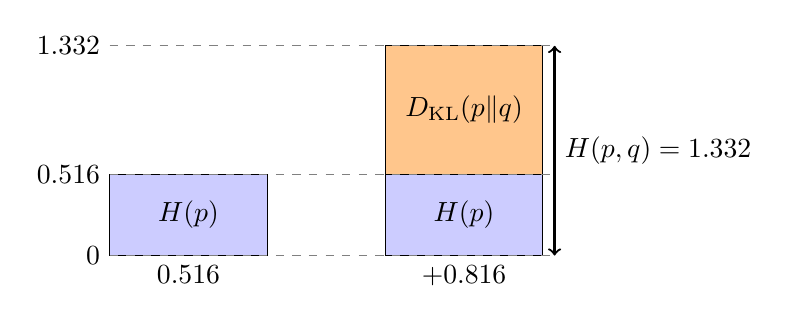
\begin{tikzpicture}[scale=1.0]
% stacked bars: H(p,q) = H(p) + KL(p||q)   (numbers from ch15_info.py)
% bar 1: H(p)
\draw[fill=blue!20] (0,0) rectangle (2,1.032);
\node at (1,0.52) {$H(p)$};
\node[below] at (1,0) {$0.516$};
% bar 2: H(p) + KL stacked = H(p,q)
\draw[fill=blue!20] (3.5,0) rectangle (5.5,1.032);
\draw[fill=orange!45] (3.5,1.032) rectangle (5.5,2.664);
\node at (4.5,0.52) {$H(p)$};
\node at (4.5,1.85) {$D_{\mathrm{KL}}(p\|q)$};
\node[below] at (4.5,0) {$+0.816$};
\draw[<->, thick] (5.65,0) -- (5.65,2.664) node[midway, right] {$H(p,q)=1.332$};
\foreach \y/\yl in {0/0, 1.032/{0.516}, 2.664/{1.332}}{
  \draw[gray, dashed] (0,\y) -- (5.6,\y);
  \node[left] at (0,\y) {\yl};
}
\end{tikzpicture}
